\section{Volume Estimation}
\label{volume estimation}
The development of Volume Estimation was split up into two phase of differing accuracy.
\subsection{Minimum Bounding Box}
\label{testing: minimum bounding box}
The bounding box approach, described in \ref{design: an initial upper bound approximation}, was useful because it allowed the calculation of a transform between point cloud space (PCS) and real world space (RWS) without the added complexity of the volume rendering technique. This transform was necessary because the Kinect stores distances in terms of pixels rather than real world measurements such as meters and it is these real world measurements that the calculated volume should be outputted in. The transform is multiplicative and as such is of the form shown in Figure \ref{testing: transform between pcs and rws}.\\

\begin{figure}[h]
\begin{center}
$Volume_{PCS} * Transform Constant = Volume_{RWS}$
\end{center}
\caption{Transform between PCS and RWS}
\label{testing: transform between pcs and rws}
\end{figure}

In order to facilitate the calculation of the transform constant, many people were scanned and their minimum bounding box calculated two ways. Firstly the box was calculated using the PARSE tool kit to give the box's volume in PCS. Secondly, the volume of the box was calculate in RWS by measuring the height, width and breadth of the person. These figures were then divided to determine the transform constant as in Figure \ref{testing: table of data used to calculate the transform constant}.\\

\begin{figure}[h]
\begin{center}
$\frac{Volume_{RWS}}{Volume_{PCS}} = Transform Constant$
\end{center}
\caption{Calculating the Transform Constant}
\label{testing: calculating the transform constant}
\end{figure}
\begin{figure}[h]
\begin{center}
  \begin{tabular}{| l | r | r | r |}
    \hline
    Person & $Volume_{RWS}$ ($m^3$) & $Volume_{PCS}$ ($units^3$) & Transform Constant \\ \hline
    Greg Corbett 	& 0.23829 & 4.70440 & 0.05065\\ \hline
    Bernard Sexton 	& 0.16200 & 4.11551 & 0.03936\\ \hline
  \end{tabular}
\end{center}
\caption{Table of Data Used to Calculate the Transform Constant}
\label{testing: table of data used to calculate the transform constant}
\end{figure}

This approach is not without a drawback, the real world bounding box must be calculated by hand, using a tape measure. Such a process is inherently error prone, as highlighted in Section \ref{spec:motivation}. However it is hoped that, by taking as large a sample as possible and averaging the transform constants, such errors can be eliminated or atleast minimized.\\

\subsection{Volume Rendering}
\label{testing: volume rendering}
This section details the testing of the volume rendering approach, discussed in Section \ref{design: a refined approach}. The method to retrieve a plane of points, all at a similar height, from a point cloud was tested by outputting the retrieved points x and z to a .csv file and plotting them using Excel. Using Excel meant that the retrieval method could be tested outside the visualization, which was at this stage untested. For testing purposes we took a slice from the approximate middle, height wise, of the Wilkinson data set \todo{(Appendix X)}, visualised in Figure \ref{fig:the wilkinson data set, visualised with an early stitching algorithm}.\\

\begin{figure}[h]
\begin{center}
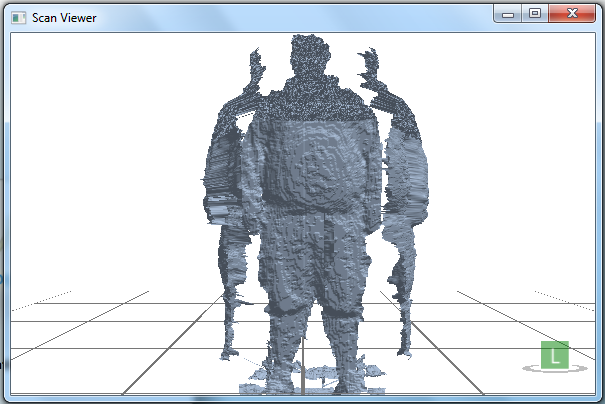
\includegraphics[scale=0.4]{./testing/wilko1} 
\end{center}
\caption{The Wilkinson data set, visualised with an early stitching algorithm.}
\label{fig:the wilkinson data set, visualised with an early stitching algorithm}
\end{figure}

Through Excel, the group achieved the following subset of the Wilkinson data set. 

\begin{figure}[h]
\begin{center}
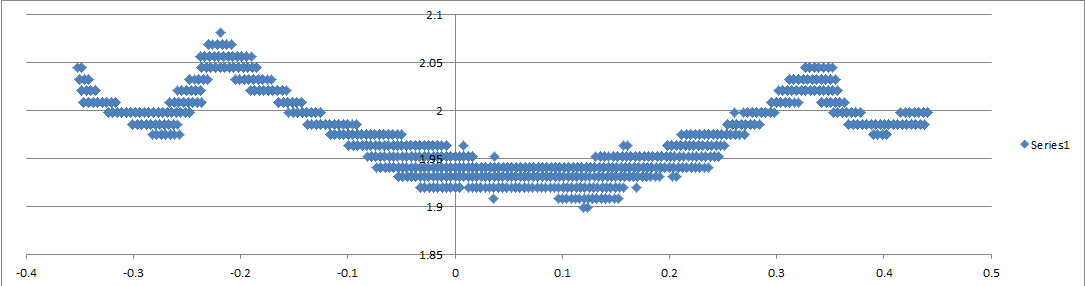
\includegraphics[scale=0.4]{./testing/wilko2} 
\end{center}
\caption{The middle plane of the Wilkinson data set.}
\label{fig:the middle plane of the Wilkinson data set.}
\end{figure}

\begin{figure}[h]
\begin{center}
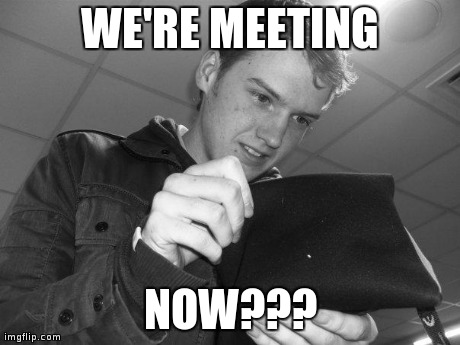
\includegraphics[scale=0.4]{./design/nathan} 
\end{center}
\caption{We're meeting now?}
\label{fig:we're meeting now?}
\end{figure}